\section{Entrega final: análisis de la implementación con herramientas de seguridad}
\label{sec:herramientas}
A diferencia del avance, la entrega final exige aplicar herramientas de seguridad para analizar la implementación. Combinamos análisis estático (SAST), análisis de composición de software (SCA), búsqueda de secretos y pruebas automatizadas. Todo se ejecuta con un solo comando, \texttt{scripts/security\_scan.sh}, y además en GitHub Actions (\path{.github/workflows/security.yml}) en cada \emph{push} y cada lunes, para detectar vulnerabilidades publicadas después de la entrega. Dependabot propone actualizaciones semanales de dependencias.

\begin{table}[H]
\centering\footnotesize
\begin{tabularx}{\textwidth}{P{2.2cm}P{1.6cm}Y Y P{1.5cm}}
\toprule
Herramienta & Tipo & Hallazgo & Corrección & Final\\
\midrule
Bandit 1.9 & SAST & 3 $\times$ B608 (SQL dinámico) en el panel, primera pasada. & Consultas fijas con parámetros con nombre. & 0\\
Bandit 1.9 & SAST & 4 $\times$ B101 en \texttt{pki.py}: la validación del certificado usaba \texttt{assert}, que \texttt{python -O} elimina; 1 $\times$ B105 (falso positivo). & Validaciones explícitas que lanzan \texttt{ValueError}. & 0 en 859 líneas\\
npm audit & SCA JS & 15 vulnerabilidades (7 altas) en dependencias de producción: \texttt{undici}, \texttt{hono}, \texttt{zod}, \texttt{systeminformation}, arrastradas por el CLI \texttt{shadcn} y el paquete \texttt{cn}. & \texttt{shadcn} pasa a desarrollo; \texttt{cn} se reemplaza por 3 líneas propias; \texttt{npm audit fix}. & 0\\
pip-audit & SCA Python & Sin vulnerabilidades conocidas en Flask, cryptography y sqlcipher3. & --- & 0\\
gitleaks 8 & Secretos & Sin alertas en el historial, pero la revisión manual halló dos contraseñas de demo en un script (sección~\ref{sec:incidente-real}). & Credenciales leídas del entorno y rotadas. & Invalidadas\\
pytest & Pruebas & 35 pruebas de S01--S06, P01 y F1--F3 sobre datos sintéticos, incluidas la revocación de sesiones y la supresión complementaria. & --- & 35/35\\
\texttt{verify\_live} & E2E HTTPS & 20 comprobaciones sobre la instancia real con TLS validado por la CA. & --- & 20/20\\
\bottomrule
\end{tabularx}
\caption{Herramientas aplicadas, hallazgos y correcciones. Reportes en \texttt{informe/evidencias/}.}
\label{tab:herramientas}
\end{table}

Tres aprendizajes surgen de este análisis. Primero, la mayor superficie de riesgo no estaba en nuestro código, sino en dependencias: un CLI de desarrollo declarado como dependencia de producción arrastraba un servidor HTTP y un SDK completos. Segundo, Bandit detectó un error sutil en código nuevo: un \texttt{assert} de seguridad desaparece con optimizaciones. Tercero, ninguna herramienta reemplaza la revisión humana: gitleaks no marcó contraseñas legibles porque no coinciden con sus patrones genéricos.

\subsection{Validación de extremo a extremo}
\label{sec:validacion}
\texttt{scripts/verify\_live.py} levanta el servidor real con el certificado de la CA propia, crea dos cuentas desechables con contraseñas aleatorias que nunca se imprimen, ejecuta solicitudes HTTPS reales y elimina las cuentas al terminar. La figura~\ref{fig:verificacion} reproduce su salida sin edición. Las 20 comprobaciones fueron correctas: cifrado y minimización de la base, sellado del ZIP, TLS 1.3 verificado, rechazo de clientes sin la CA, HSTS, control de sesión, CSRF, hash, roles, indicadores (96\,470 general; 717 en MA), validación de entrada, supresión de grupos pequeños, bloqueo por fuerza bruta, auditoría y restauración con detección de alteraciones.

\begin{figure}[H]
\centering
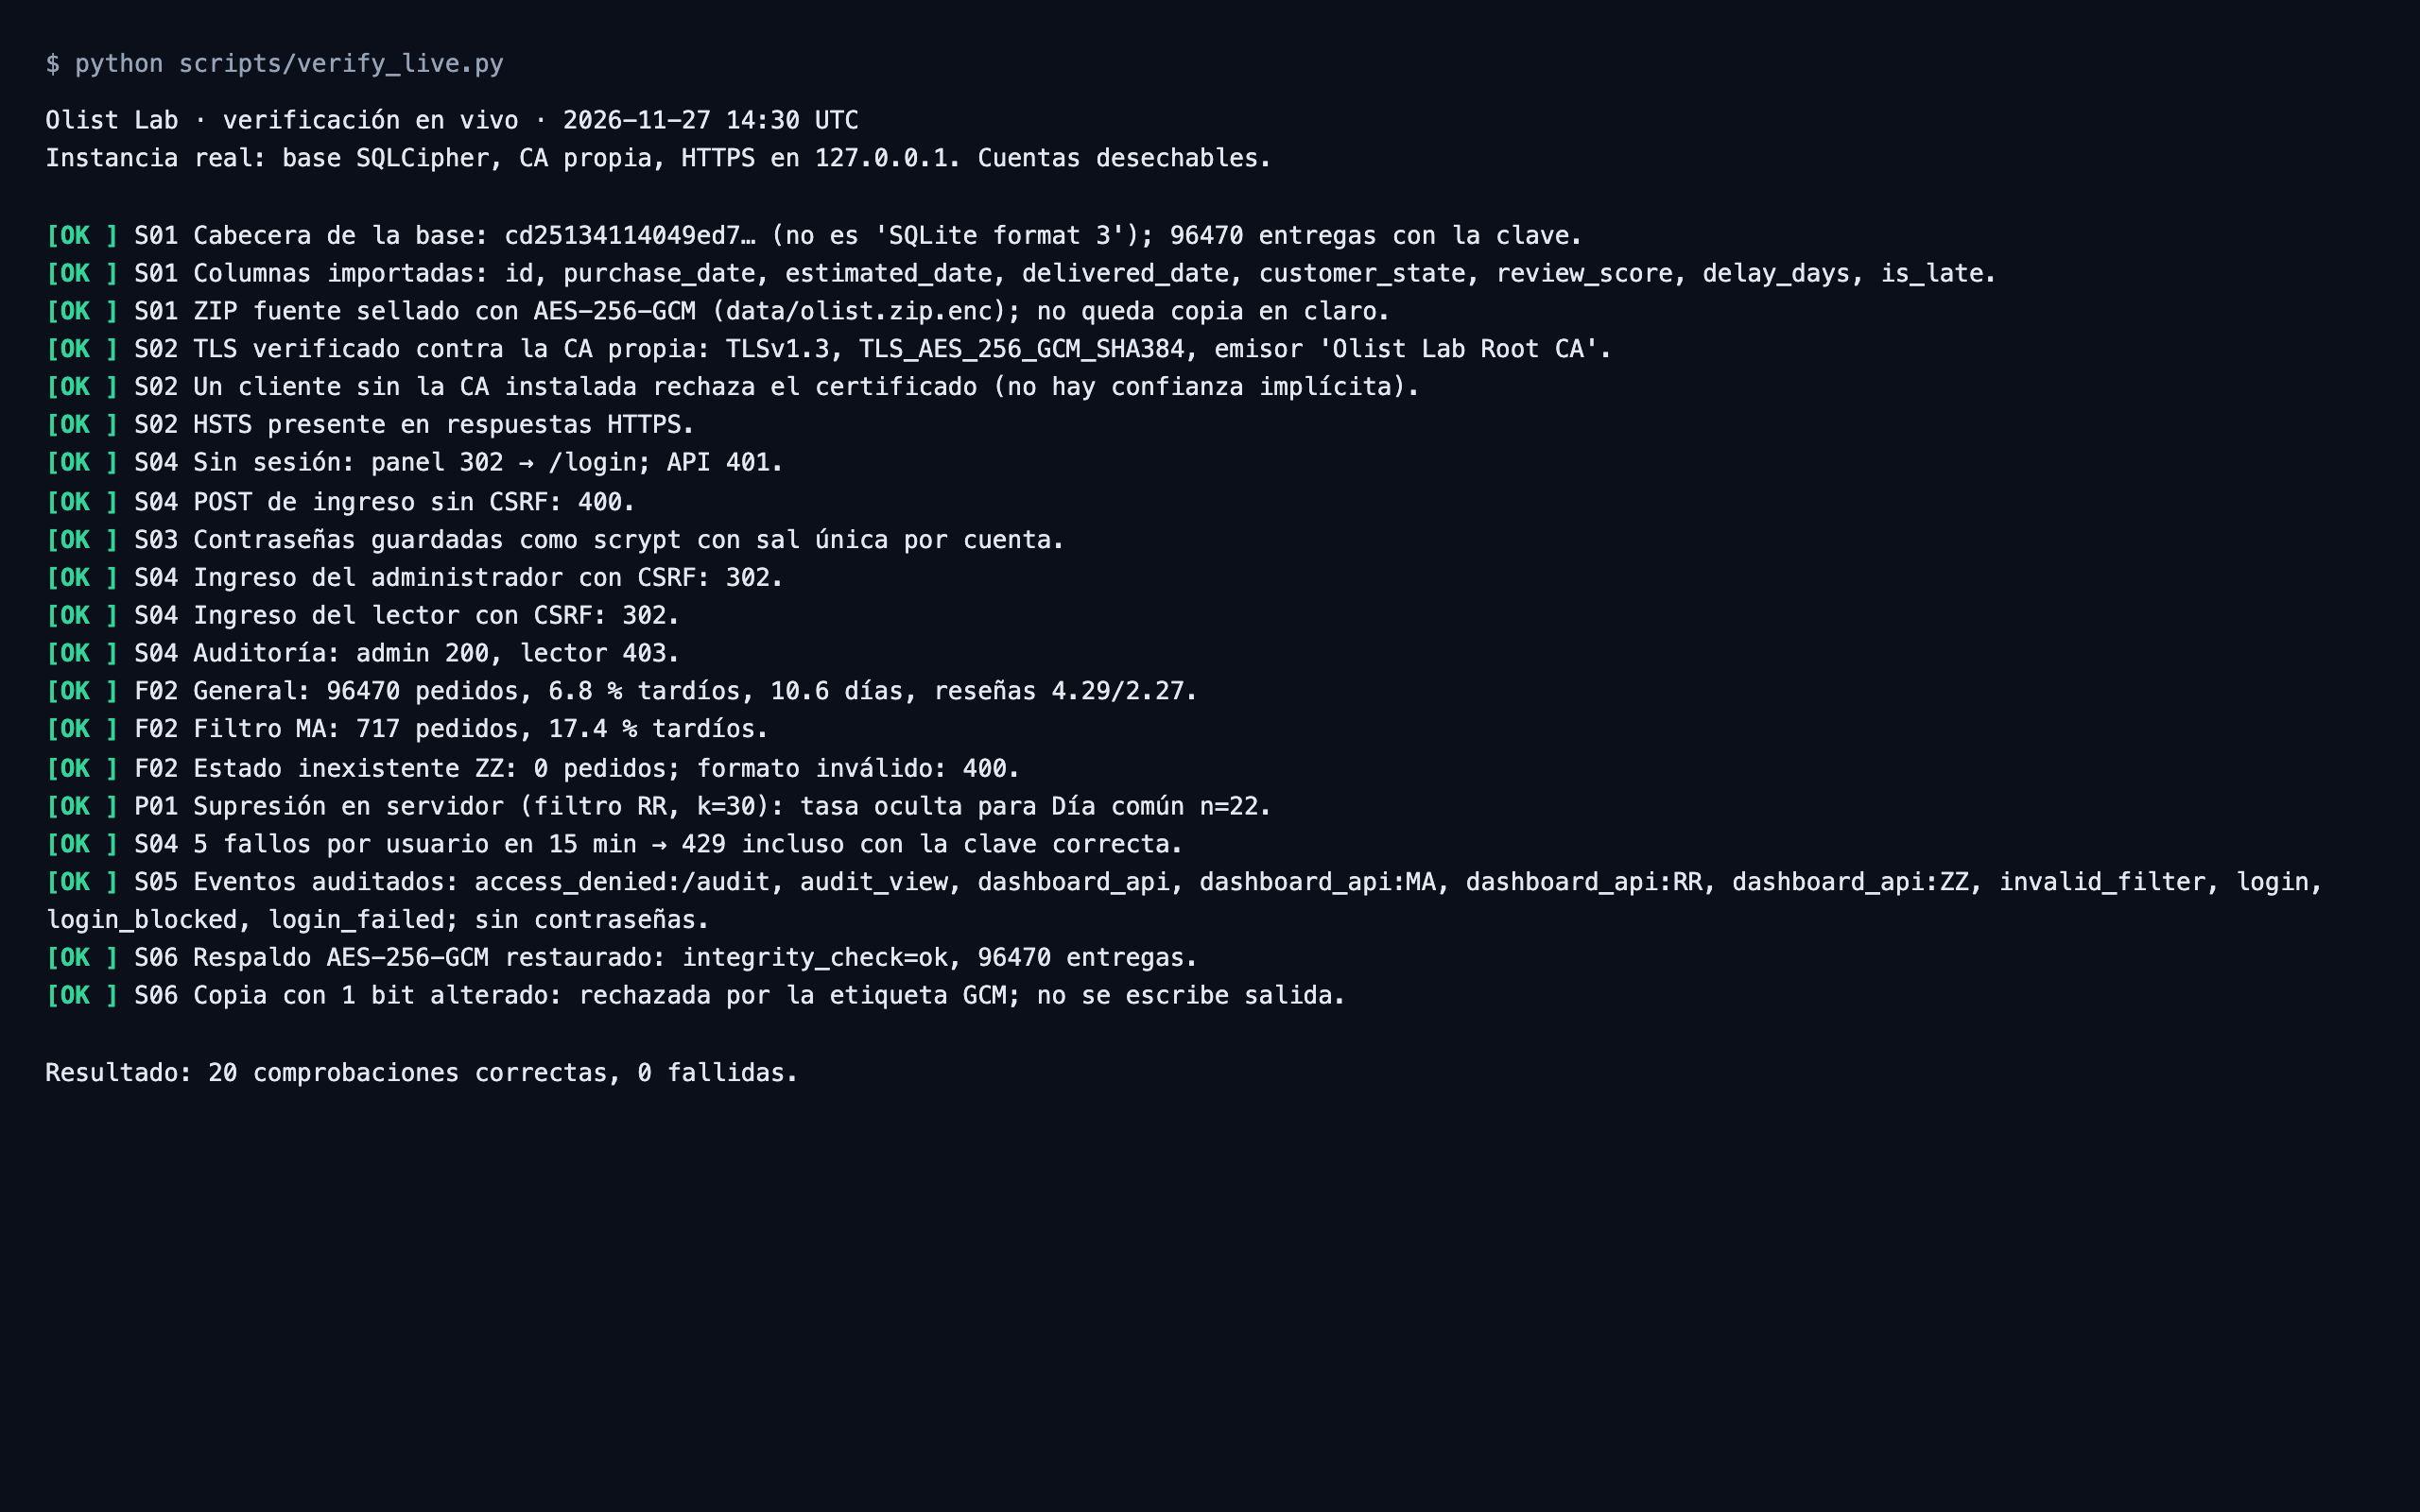
\includegraphics[width=\textwidth]{fig4_seguridad_recuperacion.png}
\caption{Salida real de \texttt{scripts/verify\_live.py} sobre la instancia de la demo.}
\label{fig:verificacion}
\fuente{\path{informe/evidencias/verificacion-final.txt}.}
\end{figure}

\section{Evaluación de Impacto en la Protección de Datos (DPIA)}
\label{sec:dpia}
\subsection{Alcance, flujo y necesidad}
Esta evaluación cubre el prototipo académico local y la publicación de su informe. Los afectados potenciales son los compradores representados en el conjunto histórico, los vendedores, los operadores cuyas cuentas y acciones quedan en auditoría y el propio equipo. El equipo gestiona el entorno de demostración; el profesor recibe el informe y presencia la demo.

El flujo va desde el ZIP de Olist y el calendario de feriados hasta la importación, la base cifrada, la API de agregados, el panel y el respaldo. Para comparar entregas se necesitan fechas, estado federado y puntuaciones. En el avance conservábamos el identificador del vendedor ``para una posible ampliación''; la DPIA concluyó que no era necesario para la finalidad, y en la entrega final \textbf{lo retiramos del importador}. Hoy la base no contiene identificadores de clientes, pedidos ni vendedores. El registro de auditoría requiere un identificador de cuenta, una acción y una marca de tiempo; la IP se guarda solo en la tabla de intentos fallidos y se borra tras 24 horas.

\subsection{Clasificación de datos y alcance normativo}
\label{sec:clasificacion}
La revisión de cabeceras identificó los campos que se indican a continuación. No inspeccionamos exhaustivamente el contenido de las reseñas ni atribuimos categorías sensibles a personas concretas. Clasificamos los datos según su posibilidad de vincularse con una persona natural y el daño que produciría su divulgación.

{\small
\begin{longtable}{@{}P{.16\textwidth}P{.40\textwidth}P{.37\textwidth}@{}}
\caption{Clasificación por etapa del tratamiento.}\\
\toprule
\textbf{Etapa} & \textbf{Campos o ejemplos} & \textbf{Clasificación y tratamiento}\\
\midrule
\endfirsthead
\toprule
\textbf{Etapa} & \textbf{Campos o ejemplos} & \textbf{Clasificación y tratamiento}\\
\midrule
\endhead
ZIP fuente & Identificadores de clientes, pedidos y vendedores, ciudad, prefijo postal, coordenadas por prefijo, fechas, valor y tipo de pago, título y texto de reseña. & Los identificadores y los atributos enlazables pueden identificar indirectamente. Importes, ubicación y comentarios merecen acceso restringido. Los comentarios pueden revelar datos sensibles si el usuario menciona, por ejemplo, información de salud. No se importan.\\
Base operativa & Identificador secuencial interno, fechas de compra, estimada y de entrega, estado federado, puntuación y retraso. & Datos transaccionales de uso interno. Sin identificadores de clientes, pedidos ni vendedores (el de vendedor se retiró en la entrega final). Se excluyen coordenadas, pagos y texto libre. Cifrada con SQLCipher.\\
Cuentas y auditoría & Usuario, rol, hash de contraseña, marca UTC y acción. & Datos de operadores y material de autenticación de acceso restringido. El nombre de cuenta puede identificar a un integrante y el registro revela su actividad. Los hashes y claves no se publican.\\
Panel e informe & Tasas y recuentos por estado, mes y feriado. & Agregados de menor riesgo. El servidor suprime grupos menores de 30 y aplica supresión complementaria para impedir deducirlos por diferencia; la interfaz no recibe esos valores.\\
\bottomrule
\end{longtable}
}

\paragraph{Perú.} Si desde Perú se tratan datos de personas identificadas o identificables, corresponde evaluar la Ley N.\textsuperscript{o} 29733 y el D. S. N.\textsuperscript{o} 016-2024-JUS según quién decide la finalidad y dónde se realiza el tratamiento \cite{leyperu,peru}. En el proyecto esto afecta especialmente el uso local del ZIP enlazable y los registros de operadores. Una fecha o un prefijo postal pueden contribuir a identificar a alguien sin pertenecer por sí solos a una categoría sensible. La ley peruana incluye, entre otros, los datos sobre salud, origen racial o étnico e ingresos económicos en su definición de datos sensibles. El monto de un pedido no mide el ingreso económico del comprador. Antes de ampliar el uso deben evaluarse la base aplicable, los avisos, la retención y el ejercicio de derechos.

\paragraph{Brasil.} El artículo 3 de la LGPD exige evaluar las conexiones territoriales del tratamiento, incluida la recolección en Brasil. El origen brasileño y la disponibilidad pública justifican revisar la procedencia y la posibilidad de identificar titulares. El artículo 4.II.b remite a los artículos 7 y 11 para el tratamiento con fines exclusivamente académicos. El artículo 5 distingue el dato personal del sensible, y el artículo 12 considera la posibilidad de revertir la anonimización con medios razonables \cite{lgpd}. En consecuencia, tratamos el ZIP y los registros vinculables como material restringido. Cualquier ampliación exige comprobar la base de tratamiento de cada conjunto, especialmente si contiene información sensible en texto libre.

\paragraph{Decisión de publicación.} Publicamos el informe, sus indicadores agregados y capturas con datos de demostración. El ZIP, las filas de la base, las claves y los logs de usuarios reales quedan fuera de la publicación. La DPIA documenta una evaluación académica de alcance y riesgos. La determinación formal del régimen aplicable y de los responsables corresponde a quienes definan un uso ulterior.


\subsection{Riesgos y controles}
Usamos una valoración cualitativa de probabilidad e impacto. Un riesgo alto exige tratamiento antes de ampliar el alcance; uno medio requiere seguimiento; uno bajo se acepta para la demo local mientras se mantengan sus controles.

\begin{table}[H]
\centering\footnotesize
\begin{tabularx}{\textwidth}{P{2.7cm}P{2.1cm}P{1.1cm}Y P{1.2cm}}
\toprule
Riesgo & Afectados & Inicial & Controles (E1 + EF) & Residual\\
\midrule
Exposición del ZIP o de las claves & Compradores, vendedores, operadores & Alto & Minimización, SQLCipher, ZIP sellado y borrado en claro, claves 0600 con carpeta separable, exclusión de Git, respaldo cifrado. & Medio-bajo\\
Reidentificación por grupos pequeños o cruces & Compradores, vendedores & Alto & Solo agregados; supresión $k=30$ \emph{en el servidor}, no solo en la interfaz; sin identificadores en la base. & Bajo\\
Exposición de cuentas y trazas & Equipo, operadores & Alto & scrypt, roles, sesión de 30 min, bloqueo por usuario e IP, retención de 180 días; contraseñas filtradas rotadas. & Medio\\
Interpretación injusta de indicadores & Vendedores, regiones, operadores logísticos & Medio & Denominadores visibles; advertencias de causalidad, cobertura temporal y reseñas ausentes. & Bajo\\
Pérdida de datos o del material de recuperación & Equipo, continuidad & Alto & Respaldo autenticado, rotación, restauración verificada, código en dos repositorios remotos. & Medio\\
Suplantación del servidor (MITM local) & Usuarios del panel & Medio & CA propia, TLS $\geq$ 1.2, HSTS; un cliente sin la CA rechaza la conexión. & Bajo\\
\bottomrule
\end{tabularx}
\caption{Riesgos, afectados y riesgo residual tras la entrega final.}
\end{table}

\subsection{Consideraciones éticas}
\paragraph{Consentimiento y finalidad.} Que el conjunto sea público no implica que los compradores hayan consentido cualquier uso. Limitamos la finalidad a un análisis académico agregado y prohibimos en la política decisiones individuales sobre compradores o vendedores.
\paragraph{Sesgo y equidad.} Las tasas por estado reflejan distancia, infraestructura y operadores, no la ``calidad'' de una región ni de sus habitantes. Las reseñas solo existen para quien decidió escribirlas; quien no reseña queda fuera del promedio, lo que puede sesgar la satisfacción observada. Por eso el panel muestra denominadores y el informe evita lenguaje causal.
\paragraph{Transparencia.} El panel indica fuentes, período y supresión de grupos pequeños; el informe documenta qué campos se excluyen y cómo se calcula cada indicador; el código y las pruebas son públicos y reproducibles.
\paragraph{Responsabilidad propia.} El incidente de credenciales (sección~\ref{sec:incidente-real}) mostró que un equipo pequeño también puede exponer secretos. Lo documentamos en lugar de ocultarlo.

\subsection{Decisión y seguimiento}
Aceptamos el riesgo residual para la demo local con datos históricos y la publicación de agregados. Antes de cualquier uso con datos reales o usuarios externos deberá reevaluarse esta DPIA: si se añaden datos, cambian los destinatarios o se despliega el backend fuera del equipo. El informe no registra consulta a afectados ni aprobación para un despliegue real.
